
% Provide a way to declare and renew a command in one command
\newcommand{\neworrenewcommand}[1]{\providecommand{#1}{}\renewcommand{#1}}

\newcommand{\drawblock}[9]{
    \neworrenewcommand{\ffoo}[1]{
           
        \foreach \i in {0,...,#8} {
            \foreach \j in {0,...,#9} {
                \foreach \k in {0,...,##1} {
                    % Only draw the visible faces
                    % Front face
                    \ifnum \i=#8
                        \draw[#7, fill=#7!50] (#1+\i*#4+#4,#2+\j*#5,#3+\k*#6) -- ++(0,#5,0) -- ++(0,0,#6) -- ++(0,-#5,0) -- cycle;
                    \fi
                    % Right face
                    \ifnum \j=#9
                        \draw[#7, fill=#7!30] (#1+\i*#4,#2+#5+\j*#5,#3+\k*#6) -- ++(#4,0,0) -- ++(0,0,#6) -- ++(-#4,0,0) -- cycle;
                    \fi
                    % Top face
                    \ifnum \k=##1
                        \draw[#7, fill=#7!20] (#1+\i*#4,#2+\j*#5,#3+#6+\k*#6) -- ++(#4,0,0) -- ++(0,#5,0) -- ++(-#4,0,0) -- cycle;
                    \fi
                    % Draw a point at each vertex
                    % \fill (#1+\i*#4,#2+\j*#5,#3+\k*#6) circle (1pt);
                }
            }
        }
    
    }
    \ffoo
}



\begin{tikzpicture}
\node[] (fig1) {  \resizebox{0.2\columnwidth}{!}{%
    \begin{tikzpicture}[node distance=0.8cm and 0.5cm, font=\sffamily , isometric view, 3d view = {140}{30}]
% coordinate system
\coordinate (O) at (0, 0, 0);


\draw[-latex] (O) -- +(1, 0,  0) node [right] {$x$};
\draw[-latex] (O) -- +(0,  1, 0) node [left] {$y$};
\draw[-latex] (O) -- +(0,  0, 1) node [above] {$z$};
\draw[-latex] (O) -- +(1, 0,  0) node [right] {$x$};
\draw[-latex] (O) -- +(0,  1, 0) node [left] {$y$};
\draw[-latex] (O) -- +(0,  0, 1) node [above] {$z$};
\drawblock{0}{0}{0}{1}{0.75}{0.5}{red}{5}{1}{5};
\drawblock{6}{0}{0}{2}{1}{3}{green}{2}{0}{0};
\drawblock{6}{1}{0}{2.5}{0.5}{3}{black}{1}{0}{0};
\drawblock{12}{0}{0}{1}{1}{1.5}{lime}{0}{0}{1};

\drawblock{0}{1.5}{0}{1}{.5}{0.25}{blue}{10}{0}{9};

\drawblock{11}{1}{0}{2}{1}{1.25}{orange}{0}{0}{1};
\drawblock{0}{1.5}{2.5}{3.6666}{.5}{0.5}{orange!40!gray}{2}{0}{0};
\drawblock{11}{1}{2.5}{2}{1}{0.5}{violet}{0}{0}{0};




% \draw[fill=gray, fill opacity=0.03] (0,0,0) -- ++(13 ,0,0) -- ++(0,2,0) -- ++(-13 ,0,0) -- cycle;
% \draw[fill=gray, fill opacity=0.03] (0,0,0) -- ++(0,0,3 ) -- ++(13 ,0,0) -- ++(0,0,-3 ) -- cycle;
% \draw[fill=gray, fill opacity=0.03] (0,0,0) -- ++(0,2,0) -- ++(0,0,3 ) -- ++(0,-2,0) -- cycle;
\draw[fill=gray, fill opacity=0.03] (13,2,3) -- ++(-13 ,0,0) -- ++(0,-2,0) -- ++(13 ,0,0) -- cycle;
\draw[fill=gray, fill opacity=0.03] (13,2,3) -- ++(0,0,-3 ) -- ++(-13 ,0,0) -- ++(0,0,3 ) -- cycle;
\draw[fill=gray, fill opacity=0.03] (13,2,3) -- ++(0,-2,0) -- ++(0,0,-3 ) -- ++(0,2,0) -- cycle;
\end{tikzpicture}
    }}; 
  \node[box, above right=0.75cm of fig1] (o1) {Loading \\  Configurations};
  \node[box, right=1cm of o1] (product) {Product \\ Selection};
  \node[aux_gene_group, fit=(o1) (product)] (group1) {};
  \node[label_node=orange, above= of group1,  minimum height=1.05cm] (Ft) {$F_t$};

  \node[label_node=orange, below= of group1, minimum height=1.05cm] (Ft1) {$F_{t+1}$};
      \tikzstyle{tline} = [draw, {Latex[length=1.5mm]}-{Latex[length=1.5mm]}]
      \tikzstyle{line} = [draw, -Latex]

  \path [tline] (o1) -- (product) ;
  \path [line] (o1) -- (Ft1) ;
  \path [line] (product) -- (Ft1) ;
  \path [line] (Ft) -- (product) ;
  \path [line] (Ft) -- (o1) ;
  
  \node [above left=0.75cm of Ft] (ul) {};
  \node [below left=0.75cm of Ft1] (dl) {};
  \node [above right=0.75cm of Ft] (ur) {};
  \node [below right=0.75cm of Ft1] (dr) {};
    \path [line] (ul) -- (Ft) ;
  \path [line] (ur) -- (Ft) ;
      \path [line] (Ft1) -- (dl) ;
  \path [line] (Ft1) -- (dr) ;

  \node[below right=0.75cm of product] (fig1) {  \resizebox{0.2\columnwidth}{!}{%
    

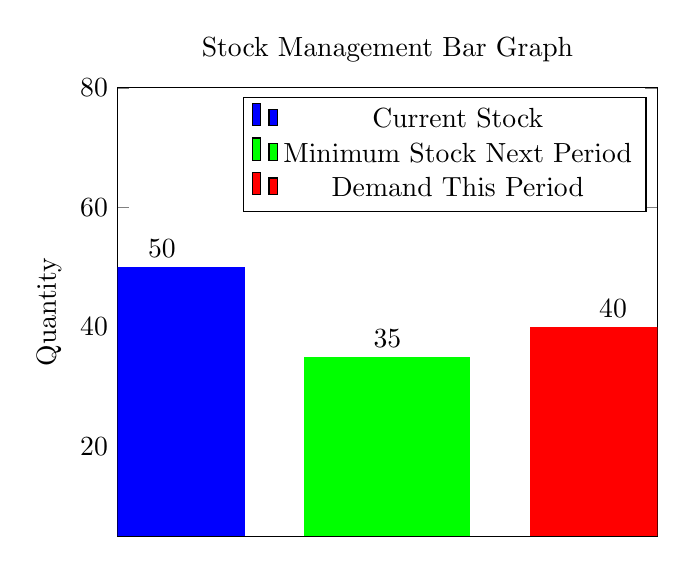
\begin{tikzpicture}
\begin{axis}[
    title={Stock Management Bar Graph},
    ybar,
    bar width=60pt,
    enlargelimits=2,
    ylabel={Quantity},
    symbolic x coords={x1,x2,x3},
    xtick=\empty, % Hides the x-axis values
    nodes near coords,
    nodes near coords align={vertical},
    every axis plot/.append style={
      fill,
      draw=none
    },
    ]
% x1 bars
\addplot [fill=blue] coordinates {(x1,50)};
\addlegendentry{Current Stock} % Legend entry for blue

% x2 bars
\addplot [fill=green] coordinates {(x2,35)};
\addlegendentry{Minimum Stock  Next Period} % Legend entry for green

% x3 bars
\addplot [fill=red] coordinates {(x3,40)};
\addlegendentry{Demand This Period} % Legend entry for red
\end{axis}
\end{tikzpicture}


    }}; 
\end{tikzpicture}